
\section{Frequenz}
\label{section:frequenz}
\begin{frame}%STARTCONTENT

\frametitle{Wechselspannung}
\begin{itemize}
  \item Die Wechselspannung im Stromnetz schwingt 50 mal in der Sekunde
  \item Die Anzahl der Schwingungen pro Sekunde nennt man Frequenz
  \item Die Einheit ist Hertz mit der Abkürzung $\text{Hz}$
  \item \qty{1}{\hertz} $\rightarrow$ 1 Schwingung pro Sekunde
  \item Das Stromnetz hat eine Frequenz von $50\ \text{Hz}$
  \end{itemize}
\end{frame}

\begin{frame}
\frametitle{Einheit Hertz}
\begin{itemize}
  \item Misst die Frequenz
  \item $1\ \text{Hz}$ $\rightarrow$1 Schwingung pro Sekunde
  \item Benannt nach dem deutschen Physiker Heinrich Rudolf Hertz
  \item Erzeugte im Jahr 1886 als erster Mensch elektromagnetische Wellen und konnte sie nachweisen
  \end{itemize}
    \pause
    $$1 \ \text{Hz} = \dfrac{1}{\text{s}}$$



\end{frame}

\begin{frame}
\only<1>{
\begin{QQuestion}{NA206}{Welche Einheit wird üblicherweise für die Frequenz einer elektrischen Schwingung verwendet?}{Hertz (Hz)}
{Meter (m)}
{Meter pro Sekunde (m/s)}
{Sekunde pro Meter (s/m)}
\end{QQuestion}

}
\only<2>{
\begin{QQuestion}{NA206}{Welche Einheit wird üblicherweise für die Frequenz einer elektrischen Schwingung verwendet?}{\textbf{\textcolor{DARCgreen}{Hertz (Hz)}}}
{Meter (m)}
{Meter pro Sekunde (m/s)}
{Sekunde pro Meter (s/m)}
\end{QQuestion}

}
\end{frame}

\begin{frame}
\only<1>{
\begin{QQuestion}{NA207}{Wenn s für Sekunde steht, gilt für die Einheit der Frequenz~...}{Hz = $\dfrac{1}{\textrm{s}}$}
{Hz = s}
{Hz = s$^2$}
{Hz = $\dfrac{1}{\textrm{s}^2}$}
\end{QQuestion}

}
\only<2>{
\begin{QQuestion}{NA207}{Wenn s für Sekunde steht, gilt für die Einheit der Frequenz~...}{\textbf{\textcolor{DARCgreen}{Hz = $\dfrac{1}{\textrm{s}}$}}}
{Hz = s}
{Hz = s$^2$}
{Hz = $\dfrac{1}{\textrm{s}^2}$}
\end{QQuestion}

}
\end{frame}

\begin{frame}
\frametitle{Hohe Schwingungen}
\begin{itemize}
  \item Im Funk wird mit viel höheren Schwingungen gearbeitet
  \item z.B. 144.000.\qty{000}{\hertz}
  \item Abkürzung: \qty{144}{\mega\hertz} (Megahertz)
  \item Einheitenvorzeichen \enquote{M} vor \enquote{Hz} gesetzt
  \item Der Wert wird mit einer Million multipliziert
  \end{itemize}
\end{frame}

\begin{frame}\begin{table}
\begin{DARCtabular}{lrr}
     Bezeichnung  & Abkürzung  & Wert   \\
     1 Kilohertz  & \qty{1}{\kilo\hertz}  & \qty{1000}{\hertz}   \\
     1 Megahertz  & \qty{1}{\mega\hertz}  & \qty{1000000}{\hertz}   \\
     1 Gigahertz  & \qty{1}{\giga\hertz}  & \qty{1000000000}{\hertz}   \\
\end{DARCtabular}
\caption{Kurzschreibweise für große Frequenzen}
\label{n_frequenz_einheitenvorzeichen}
\end{table}
\end{frame}

\begin{frame}
\only<1>{
\begin{QQuestion}{NA212}{\qty{144000000}{\Hz} entspricht ...}{\qty{1,44}{\kHz}}
{\qty{144}{\kHz}}
{\qty{1,44}{\GHz}}
{\qty{144}{\MHz}}
\end{QQuestion}

}
\only<2>{
\begin{QQuestion}{NA212}{\qty{144000000}{\Hz} entspricht ...}{\qty{1,44}{\kHz}}
{\qty{144}{\kHz}}
{\qty{1,44}{\GHz}}
{\textbf{\textcolor{DARCgreen}{\qty{144}{\MHz}}}}
\end{QQuestion}

}
 \end{frame}

\begin{frame}
\frametitle{Frequenzen Klasse N}
In der Klasse~N dürfen drei Frequenzbereiche verwendet werden

\begin{itemize}
  \item \qty{28}{\mega\hertz} bis \qty{29,7}{\mega\hertz}
  \item \qty{144}{\mega\hertz} bis \qty{146}{\mega\hertz}
  \item \qty{430}{\mega\hertz} bis \qty{440}{\mega\hertz}
  \end{itemize}
    \pause
    In der Klasse~E und A kommen weitere Frequenzbereiche hinzu



\end{frame}

\begin{frame}
\only<1>{
\begin{QQuestion}{VD723}{In welchen Frequenzbereichen ist für Funkamateure mit Zulassung für die Klasse~N Sendebetrieb erlaubt?}{\qtyrange{28}{29.7}{\MHz}, \qtyrange{144}{146}{\MHz}, \qtyrange{430}{440}{\MHz}}
{\qtyrange{7}{7.2}{\MHz}, \qtyrange{14}{14.35}{\MHz}, \qtyrange{1240}{1300}{\MHz}}
{Auf allen dem Amateurfunk in Deutschland zugewiesenen Kurzwellen-Frequenzbereichen}
{Auf allen dem Amateurfunk in Deutschland zugewiesenen Frequenzbereichen oberhalb der Kurzwelle}
\end{QQuestion}

}
\only<2>{
\begin{QQuestion}{VD723}{In welchen Frequenzbereichen ist für Funkamateure mit Zulassung für die Klasse~N Sendebetrieb erlaubt?}{\textbf{\textcolor{DARCgreen}{\qtyrange{28}{29.7}{\MHz}, \qtyrange{144}{146}{\MHz}, \qtyrange{430}{440}{\MHz}}}}
{\qtyrange{7}{7.2}{\MHz}, \qtyrange{14}{14.35}{\MHz}, \qtyrange{1240}{1300}{\MHz}}
{Auf allen dem Amateurfunk in Deutschland zugewiesenen Kurzwellen-Frequenzbereichen}
{Auf allen dem Amateurfunk in Deutschland zugewiesenen Frequenzbereichen oberhalb der Kurzwelle}
\end{QQuestion}

}
 \end{frame}

\begin{frame}
\frametitle{Oszillator}
\begin{itemize}
  \item Ein Oszillator erzeugt elektrische Schwingungen in einem Funkgerät
  \item Beim Senden werden die Schwingungen auf die Antenne geleitet und als Funkwellen abgestrahlt
  \end{itemize}

\end{frame}

\begin{frame}
\only<1>{
\begin{QQuestion}{ND201}{Was verstehen Sie unter einem \glqq Oszillator\grqq ?}{Es ist ein Messgerät zur Anzeige von Schwingungen.}
{Es ist ein sehr schmales Filter.}
{Es ist ein Schwingungserzeuger.}
{Es ist ein Hochfrequenzverstärker.}
\end{QQuestion}

}
\only<2>{
\begin{QQuestion}{ND201}{Was verstehen Sie unter einem \glqq Oszillator\grqq ?}{Es ist ein Messgerät zur Anzeige von Schwingungen.}
{Es ist ein sehr schmales Filter.}
{\textbf{\textcolor{DARCgreen}{Es ist ein Schwingungserzeuger.}}}
{Es ist ein Hochfrequenzverstärker.}
\end{QQuestion}

}
\end{frame}

\begin{frame}
\frametitle{Frequenzmessung}
\begin{columns}
    \begin{column}{0.48\textwidth}
    
\begin{figure}
    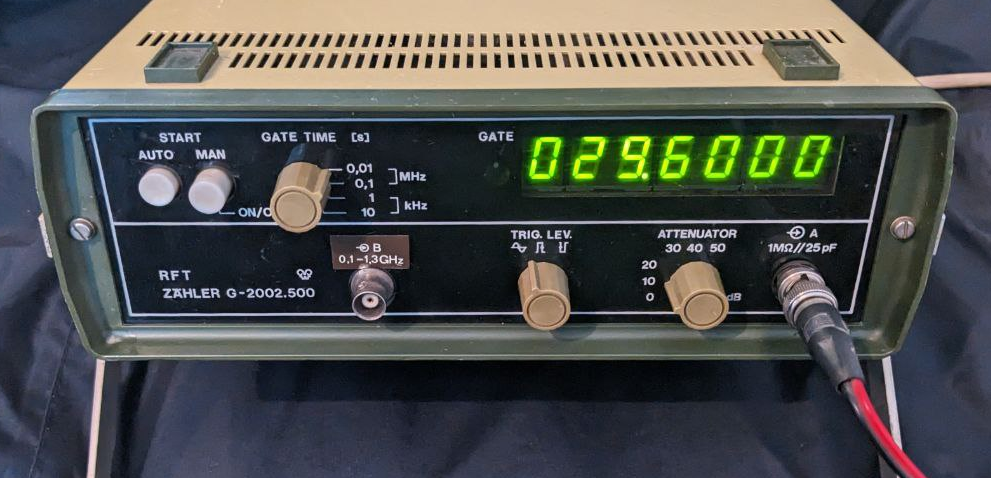
\includegraphics[width=0.85\textwidth]{foto/150}
    \caption{\scriptsize Frequenzzähler, der \qty{29,6}{\mega\hertz} misst}
    \label{frequenz_frequenzzaehler}
\end{figure}

    \end{column}
   \begin{column}{0.48\textwidth}
       \begin{itemize}
  \item Die genaue Sendefrequenz muss bekannt sein
  \item Die Messung erfolgt mit einem Frequenzzähler
  \item Zum Abgleich der Anzeige am Funkgerät
  \end{itemize}

   \end{column}
\end{columns}

\end{frame}

\begin{frame}
\only<1>{
\begin{QQuestion}{NI301}{Mit welchem Gerät kann die Sendefrequenz eines Senders gemessen werden?  }{Frequenzzähler}
{SWR-Meter}
{HF-Voltmeter}
{S-Meter}
\end{QQuestion}

}
\only<2>{
\begin{QQuestion}{NI301}{Mit welchem Gerät kann die Sendefrequenz eines Senders gemessen werden?  }{\textbf{\textcolor{DARCgreen}{Frequenzzähler}}}
{SWR-Meter}
{HF-Voltmeter}
{S-Meter}
\end{QQuestion}

}
\end{frame}%ENDCONTENT
